The initial protocol and compiled checkpoint were saved privately, reopened and hash-verified before confirmation. Development used only the allowed seed range 1--8 and hand-written analytic examples. A development run encountered disk exhaustion and remains labelled incomplete; its raw records were losslessly compressed with original hashes. Streaming gzip was introduced before the final source freeze. A fresh six-world smoke campaign and focused checks qualified the revised serialization. No holdout seed was opened to repair the implementation or choose a favorable result.

The final protocol fixes 32 seeds, 12 epochs and eight conditions, yielding 3,072 matched worlds. Seven methods yield 21,504 method records. Every method receives the same current mission and previous diagnostic report. Invocation order rotates; a copied source tree and separate worker execute the complete native replica. The exact and adaptive experts are separately implemented direct enumerators; the simple greedy comparator is intentionally sufficient when the model permits it.

\begin{table}[H]\small\renewcommand{\arraystretch}{1.13}
\begin{tabularx}{\textwidth}{@{}p{0.27\textwidth}X@{}}\toprule
Method & Comparison being tested\\\midrule
Conservative idea operationalization & Best allocation while recalibrating before every occupied sample tick; capability-removal baseline.\\
Disclosed implementation & The same native shared-calibration plan; no extra external receipt inspection or signed ledger service.\\
Verified artifact & Native plan plus complete external inspection and scoped signed evidence.\\
Complete clone & Copied native/evidence source, fresh execution, separate ephemeral key and ledger, equivalent rights and inputs.\\
Independent exact expert & Separately authored exhaustive optimum for the public stationary planning model; signed replay evidence.\\
Conventional greedy & Value-first calibration reuse; independently replayed outcomes and signed evidence.\\
Adaptive expert & Exhaustive search using the previous epoch's delayed bias profile; signed replay evidence.\\\bottomrule
\end{tabularx}
\caption{The conservative baseline isolates the enabling restriction. The complete clone and conventional experts test whether that benefit is exclusively attributable to the artifact.}
\end{table}

The conditions are ordinary operation, doubled sample capacity, one-tick calibration validity, hidden measurement drift, public demand-weight drift after six epochs, shared stochastic slot failures, zero-duration calibration, and eight repeated evidence inspections. The first epoch has no prior diagnostic report. An instrument slot failure and an invalid measurement both consume resources. Every method's true synthetic output is scored identically.

The one primary contrast is the ordinary-condition useful-output improvement of the verified artifact over the conservative baseline, with a predeclared practical margin of 5\%. The independent unit is the seed: twelve epochs are averaged within seed, then 32 seed clusters are resampled 10,000 times. We report paired percentile 95\% bootstrap intervals. Other conditions, cost comparisons and trajectories are descriptive stress analyses. We do not treat thousands of dependent jobs as independent observations or infer a permanent moat from a confidence interval.

Budget limits are one active scientific policy at a time, a 30-minute campaign, a one-million native logical-work budget per plan, 20-second native request leases and 512-MiB heaps per worker. Both workers may remain resident; the requests are sequential. Enumeration is finite and the entire campaign is subject to the outer limit. Original failed invocations and incomplete development evidence remain in the archive.

\subsection{Productive output and the copying result}
\MainResults

Independent replay verifies all 21,504 outcomes, 15,360 signatures and 15,360 ledgers with zero audit errors. A separate closed-form calculation checks 18,432 nominal objectives without importing either optimizer. All 48 retained full native completions pass the unchanged source-bound inspector. Zero method noncompletions does not mean zero measurement failures: the verified artifact has failed realized measurements in 583 worlds, retained in its outcome and resource accounts.
\ResultsTable

\begin{figure}[H]\centering
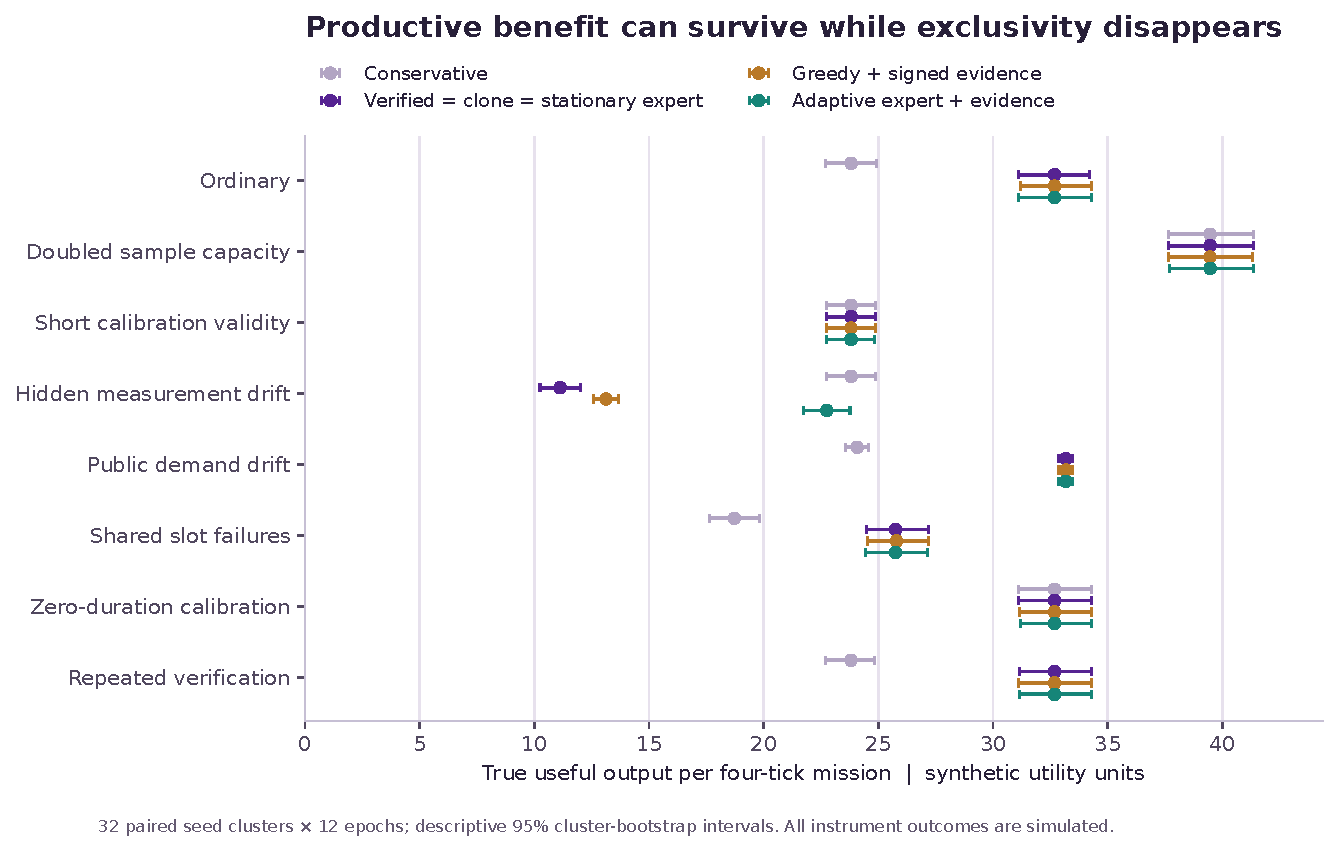
\includegraphics[width=\textwidth]{../figures/condition-outcomes.pdf}
\caption{Measured software outcomes in synthetic worlds. Each point averages 32 seed clusters of 12 epochs; intervals are descriptive cluster-bootstrap intervals. Native verified, complete clone and stationary exact-expert outputs coincide. A positive difference from the conservative restriction does not establish superiority to conventional shared-calibration scheduling.}
\end{figure}

\subsection{Drift reveals what the proof did not establish}
\DriftResults

\begin{figure}[H]\centering
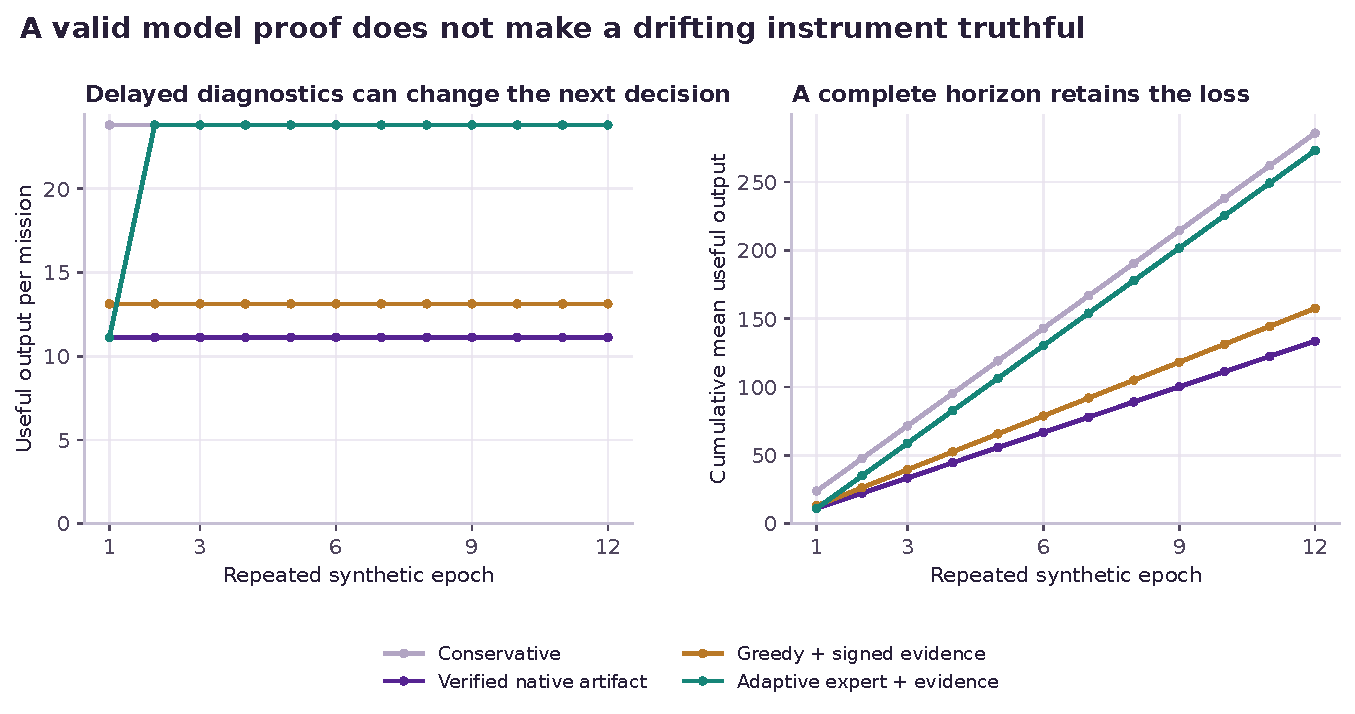
\includegraphics[width=\textwidth]{../figures/drift-and-time.pdf}
\caption{All twelve repeated epochs are shown. The adaptive competitor can use the previous epoch's perfect delayed diagnostic report; the first epoch cannot. The diagnostic channel consumes separately counted auxiliary acquisitions. These are short synthetic missions, not observations of commercial duration or physical calibration reliability.}
\end{figure}

\subsection{The sufficient comparator can be cheaper}
\ComputeResults
The experiment does not award the artifact a benefit simply for carrying more machinery. The independent expert can rebuild the finite allocation and verify its outputs; the simple greedy scheduler is a useful substitute when its assumptions fit. Native proof export may serve an integration or audit purpose, but an unmeasured purpose cannot be booked as an observed gain.

\begin{figure}[H]\centering
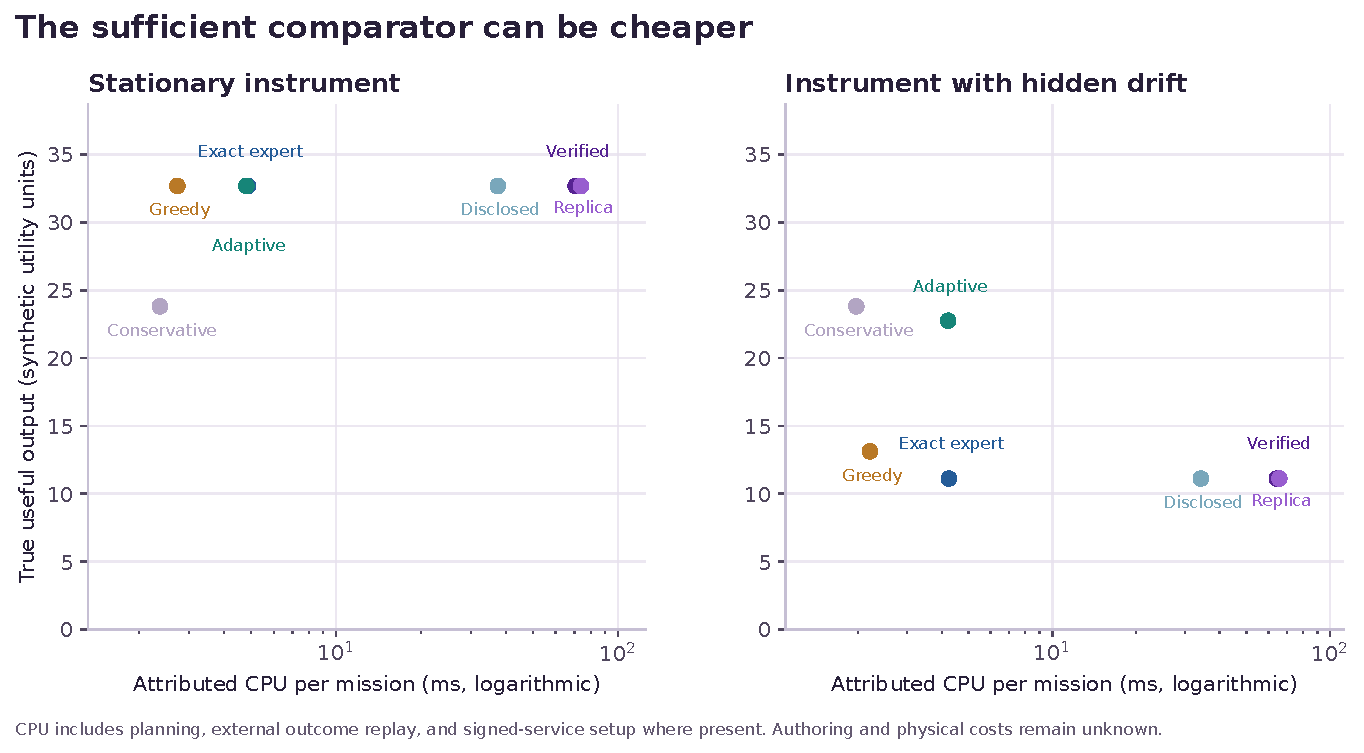
\includegraphics[width=\textwidth]{../figures/output-compute.pdf}
\caption{Output versus measured attributed CPU per mission, including the common external evaluator and the signed-service setup where present. Native optimizer/proof work is separately itemized. The cheaper adequate comparators are retained. Costs omit unknown authoring labor, actual instrument cost and commercial integration.}
\end{figure}
